\chapter{Mathematische Formeln und Anwendung} \label{chap:mathematische-formeln}

\section{Multiple Sequence Alignment mit MAFFT} \label{sec:mafft-mathematik}

MAFFT wird zur Erstellung von Multiplen Sequenzalignments (\gls{msa}) genutzt. Durch eine Fourier-Transformation wird eine effiziente Berechnung dabei ermöglicht. Die Qualität eines Alignments wird durch eine Punktzahl $\mathcal{S}$ bewertet, die die Übereinstimmung zwischen den Sequenzen quantifiziert:

\begin{align}
    \mathcal{S} = \sum_{i=1}^n \sum_{j=i+1}^n w_{ij} \cdot \text{Score}(i, j)
\end{align}

Hierbei ist $w_{ij}$ ein Gewichtungsfaktor, der die Relevanz des Vergleichs zwischen Sequenz $i$ und Sequenz $j$ angibt, und $\text{Score}(i, j)$ ist die Ähnlichkeit zwischen den beiden Sequenzen basierend auf Substitutionsmatrizen wie BLOSUM oder PAM.

\paragraph{Transformation in das Frequenzspektrum}
MAFFT nutzt die Fourier-Transformation zur effizienten Berechnung der Ähnlichkeiten zwischen Sequenzen. Die Transformation ist definiert als:

\begin{align}
    \mathcal{F}(k) = \sum_{n=0}^{N-1} x(n) \cdot e^{-i \frac{2\pi k n}{N}}
\end{align}

Hierbei ist $\mathcal{F}(k)$ das Frequenzspektrum der Sequenz, $x(n)$ die diskrete Funktion der Sequenz an Position $n$, $N$ die Länge der Sequenz und $i$ die imaginäre Einheit. Die resultierenden Distanzwerte werden in einer Distanzmatrix $\mathcal{D}(i, j)$ zusammengefasst:

\begin{align}
    \mathcal{D}(i, j) = 1 - \frac{\sum_{k=1}^L \delta(x_k^i, x_k^j)}{L}
\end{align}

wobei $\delta(x_k^i, x_k^j)$ 1 ist, wenn die Aminosäuren an Position $k$ in Sequenz $i$ und $j$ identisch sind, sonst 0. $L$ ist die Länge des Alignments.

\paragraph{Praktische Anwendung:}
MAFFT kann auf der Kommandozeile folgendermaßen ausgeführt werden:
\begin{verbatim}
    mafft [arguments] input > output
\end{verbatim}

\begin{figure}[H]
    \centering
    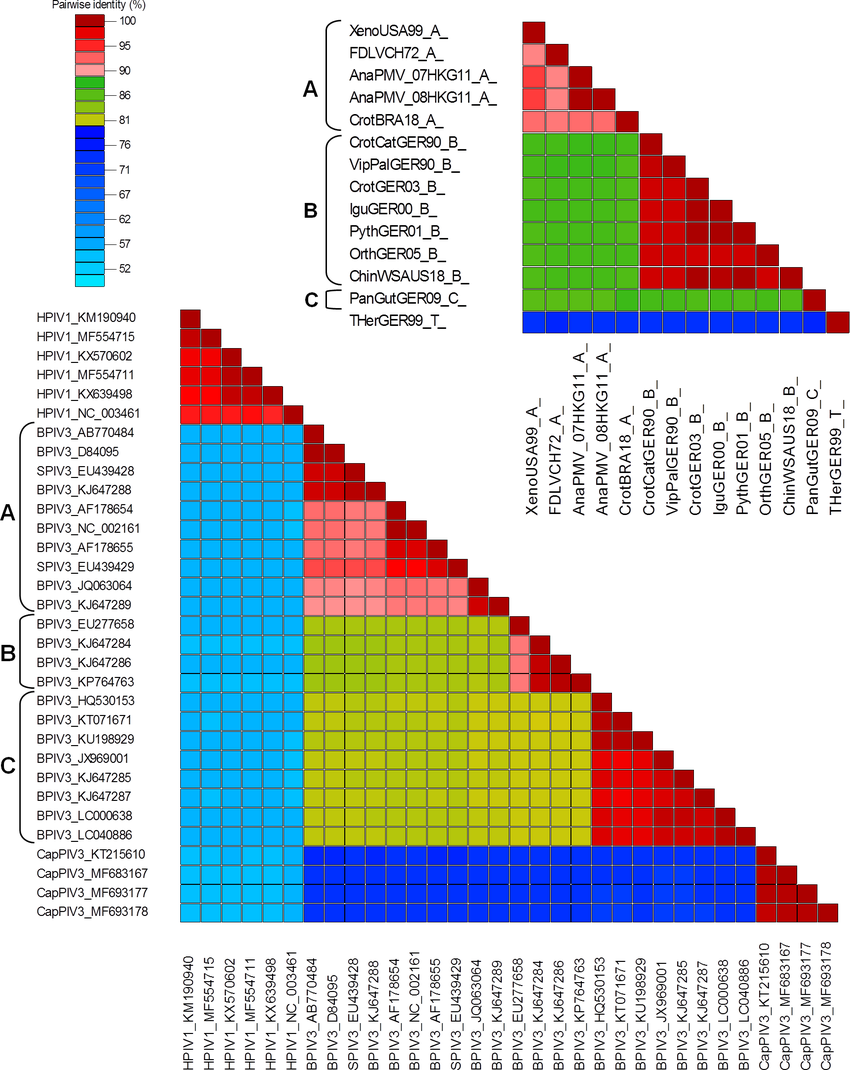
\includegraphics[width=.5\textwidth]{/workspaces/seminar-bioinformatik/images/mafft_distance_matrix.png}
    \caption{Beispiel einer Distanzmatrix nach der Anwendung von MAFFT. \autocite{peesThreeGeneticallyDistinct2019}}
    \label{fig:mafft-distance-matrix}
\end{figure}

\section{Maximum-Likelihood-Methode und Substitutionsmodell} \label{sec:maxlikelihood}

Die Maximum-Likelihood-Methode zielt darauf ab, die Baumtopologie $T$ zu finden, die die Wahrscheinlichkeit der beobachteten Daten $D$ maximiert, gegeben ein Modell $M$:

\begin{align}
    \mathcal{L}(M) = P(D \mid M) = \prod_{i=1}^{n} P(d_i \mid M)
\end{align}

Hierbei ist $\mathcal{L}(M)$ die Likelihood des Modells, und $P(d_i \mid M)$ die Wahrscheinlichkeit der Daten an Position $i$, gegeben das Modell $M$.

\paragraph{Substitutionsmodell GTR+I+G}
Das GTR+I+G-Modell berücksichtigt:
\begin{itemize}
    \item \textit{Unterschiedliche Substitutionsraten} zwischen Nukleotiden.
    \item \textit{Invariante Positionen} (I), die konserviert bleiben.
    \item \textit{Rate-Heterogenität} (G), die durch eine Gamma-Verteilung modelliert wird.
\end{itemize}

Die Gamma-Verteilung $\Gamma$ beschreibt die Variabilität der Mutationsrate an verschiedenen Positionen:

\begin{align}
    \Gamma(\alpha, \beta) = \frac{\beta^\alpha}{\Gamma(\alpha)} x^{\alpha - 1} e^{-\beta x}
\end{align}

wobei $\alpha$ und $\beta$ die Form- und Skalierungsparameter sind.

\paragraph{Praktische Anwendung:}
Die Baumrekonstruktion mit IQ-TREE kann durch folgenden Befehl durchgeführt werden:
\begin{verbatim}
iqtree -s aligned_sequences.fasta -m GTR+I+G -bb 1000
\end{verbatim}
Dabei führt IQ-TREE 1.000 Bootstrapping-Wiederholungen durch.

\section{Berechnung der Root-Mean-Square Deviation (RMSD)} \label{sec:rmsd-berechnung}

Die Root-Mean-Square Deviation (\gls{rmsd}) misst die durchschnittliche Distanz zwischen entsprechenden Atomen zweier Proteinstrukturen nach optimaler Überlagerung:

\begin{align}
    \text{RMSD} = \sqrt{\frac{1}{N} \sum_{i=1}^N \| \mathbf{p}_i - \mathbf{q}_i \|^2}
\end{align}

Dabei sind $\mathbf{p}_i$ und $\mathbf{q}_i$ die Koordinaten des $i$-ten Atoms in den beiden Strukturen, und $N$ ist die Gesamtzahl der Atome.

\paragraph{Beispiel zur RMSD-Berechnung:}
Gegeben sind zwei Atome mit den Koordinaten $\mathbf{p}_i = (1, 2, 3)$ und $\mathbf{q}_i = (2, 3, 4)$:

\begin{align}
    \| \mathbf{p}_i - \mathbf{q}_i \| = \sqrt{(2-1)^2 + (3-2)^2 + (4-3)^2} = \sqrt{3}.
\end{align}

Die RMSD ergibt sich durch das Mittel der quadrierten Abweichungen über alle Atome.